\documentclass[letterpaper, 10 pt, conference]{ieeeconf}

\usepackage[draft]{graphics} %DRAFT MODE
% \usepackage{graphics}

\let\labelindent\relax
\IEEEoverridecommandlockouts
\overrideIEEEmargins

%floats and figures
\usepackage{graphics}
\usepackage[pdftex]{graphicx}
\usepackage[font={small}]{caption}
\usepackage{subcaption}
%\usepackage[center]{subfigure} %DONT USE BOTH SUBCAPTION AND SUBFIGURE
%\DeclareGraphicsExtensions{.pdf,.png,.jpg}
%\usepackage{overpic}
%\usepackage[rightcaption]{sidecap}
%\usepackage{pbox}

%Math Stuff
\usepackage{mathtools}
\usepackage{amsmath, amssymb, amscd}
%\usepackage{ wasysym } %special symbols
\usepackage{amsfonts}
\usepackage{mathptmx}       % selects Times Roman as basic font
\DeclareMathAlphabet{\mathcal}{OMS}{lmsy}{m}{n}
\DeclareSymbolFont{largesymbols}{OMX}{cmex}{m}{n}
\usepackage{algorithm}
\usepackage{algorithmicx}
%\usepackage{algorithm}
%\usepackage{algpseudocode}
% \usepackage[ruled,vlined,linesnumbered]{algorithm2e}
\usepackage{ textcomp } %for getting text tilde

%Table Stuff
\usepackage{array} %for table entries to be in center of cell
\usepackage{tabularx}
\usepackage{multicol}
\usepackage{multirow}

%DOCUMENT WIDE
\usepackage{times} % assumes new font selection scheme installed
\usepackage{xspace}
\usepackage[english]{babel} %for hyphenation rules
\usepackage{flushend}%balance columns on last page
\usepackage{fixltx2e} %fix latex issue across versions
\usepackage{bm}
\usepackage{units}

\usepackage{makeidx}
\usepackage{enumitem}
\usepackage[yyyymmdd,hhmmss]{datetime}
\usepackage[english]{babel}

%Bibliography and cross-ref
\makeatletter
\let\NAT@parse\undefined
\makeatother
\usepackage[numbers, sort&compress]{natbib}
\renewcommand{\bibfont}{\footnotesize}
% \usepackage{cite} %DONT USE NATBIB AND CITE TOGETHER

%hyperlinking
\usepackage{url}
\makeatletter
\g@addto@macro{\UrlBreaks}{\UrlOrds}
\makeatother
\usepackage{color}
\usepackage[usenames,dvipsnames, table]{xcolor}
\usepackage[pdfborder={0 0 0.5}]{hyperref}
\hypersetup{
    colorlinks=true,
    linkcolor=blue,
    citecolor=black,
    filecolor=cyan,
    urlcolor=blue
}


%=======U S E R  D E F I N E D  M A C R O S=======
% \newcommand{\bibhref}[2]{#2}
\newcommand{\todo}[1]{\textcolor{red}{[#1]}}
\newcommand{\tocite}{\textcolor{red}{[cite]}}
\newcommand{\ignore}[1]{}

% Usage:
% \figlabel{myfigure} creates \label{fig:myfigure}
% \figref{myfigure} references it
\newcommand{\figlabel}[1]{\label{fig:#1}}
\newcommand{\figref}[1]{Figure~\ref{fig:#1}}

% Usage:
% \seclabel{mysection} creates \label{sec:mysection}
% \secref{mysection} references it
\newcommand{\seclabel}[1]{\label{sec:#1}}
\newcommand{\secref}[1]{Section~\ref{sec:#1}}

% Usage:
% \tablabel{mytable} creates \label{tab:mytable}
% \tabref{mytable} references it
\newcommand{\tablabel}[1]{\label{tab:#1}}
\newcommand{\tabref}[1]{Table~\ref{tab:#1}}

% use this command instead of writing "da Vinci" so it's never split 
\newcommand{\davinci}{da~Vinci\xspace}


\usepackage{blindtext}

%===============================================================

\title{\LARGE \bf
Autonomous Continuous Suturing on dVRK with Curvature Constrained Trajectory Optimization under Needle Pose Uncertainty
% Autonomous Continuous Suture under Uncertainty with Trajectory Optimization for  on the da Vinci Research Kit. 
}

\author{%
Siddarth Sen*$^{1}$, 
Animesh Garg*$^{2}$,
David Gealy$^{3}$,
Yiming Jen$^{1}$, 
Stephen McKinley$^{3}$,
% W Douglas Boyd$^{4}$,
Ken Goldberg$^{2}$%
\thanks{\hrule \vspace{3pt} * These authors contributed equally to the paper}
\thanks{The authors are with University of California, Berkeley CA USA}%
\thanks{$^{1}$EECS, \texttt{\{siddarthsen, yjen\}@berkeley.edu}}%
\thanks{$^{2}$IEOR \& EECS, \texttt{\{animesh.garg, goldberg\}@berkeley.edu}}%
\thanks{$^{3}$Mechanical Engineering, \texttt{\{dgealy, mckinley\}@berkeley.edu}}%
%Authors are with the Department of Electrical Engineering and Computer Sciences, University of California at Berkeley, CA, USA.}
}

\begin{document}

\maketitle
\thispagestyle{empty}
\pagestyle{empty}

%==START SECTION==============================
\begin{abstract}
Suturing is a frequently occurring yet challenging and time consuming task during Robot Assisted Minimally Invasive Surgery. And automation of suturing has the potential reduce both time and dexterity required for this subtask. 
This work focuses on continuous suturing, a technique that involves multiple throws of suture with a knot only at the end and is often used in procedures such as anastomosis requiring long-wound closures.
However, the some of the challenges in automation of such a complex task are modelling of needle-tissue interactions, maintaining needle orientation while grasping and hand-off and difficulty in real-time needle pose estimation. Moreover, careful hierarchical planning is required for robust long-term execution of continuous suturing. 

We propose a framework that enables automation of the continuous suturing task. We build on state-of-the-art autonomous task segmentation algorithms for suturing to construct finite state machine~(FSM) with sub-tasks. 
Our system parametrizes each problem instance with suture width, suture depth and a spline along the wound. It then computes the number of suture throws required and pair of entry-exit points along with the best needle size. Each suture throw is modeled as trajectory planning along with needle pose estimation through a joint belief space optimization problem.
We use a best-practice reference trajectory as an initialization to sequential convex programming solver. Furthermore, we have devised a novel needle alignment attachment for the gripper jaw that passively guides the needle into a known pose upon gripper closure. The device improves needle hand-off accuracy by \todo{x\%} compared to using current needle driver; and hence reduces the need for re-alignment before pushing needle in tissue.  

We demonstrate our approach on a 4-throw continuous suturing task with dVRK on a planar tissue model that contains skin and subcutaneous fat similar to task in Fundamental Skills of Robotic Surgery, and evaluate performance with OSATS as well as against Suturing demonstrations from the JIGSAWS dataset~\cite{gao2014jhu} on Accuracy \& Time. Our results indicate that we are \todo{xx} slower than experts and \todo{xx} with novices. We also evaluate the performance on a more complex suturing model with flexible vertical flaps and evaluate performance on time to completion and rate of success.\\
\todo{A tad too long--trim text, move to intro}

% This study formulates the problem of trajectory planning
% along with needle pose estimation as a joint belief space optimization problem. The framework allows autonomous discovery of a robust path in presence a asymmetric uncertainty model for needle manipulation. Furthermore, the system uses a reference trajectory modelled with best-practices in surgical training to provide improved initialization for the sequential convex programming solver.

% Our system uses user input for providing wound outline and then parametrizes the problem automatically compute 
\end{abstract} 

%this begin is only for subfile compilation
\documentclass[0-suturing.tex]{subfiles}
\begin{document}

%==START SECTION==============================
\section{Introduction}
\label{sec:intro}
%============================================
Robot-assisted surgical systems in Minimally Invasive Surgery (RMIS)
have facilitated pairing of human surgical expertise with the precision and repeatability of robots. Intuitive Surgical's da Vinci Robotic Surgical Assistant, a type of RSA, facilitated over $570,000$ procedures worldwide in $2014$ with $3000$ systems~\cite{AnnualReport2014}.
In spite of the growing prevalence of the robot-assisted minimally invasive surgery (RMIS), manual control under tele-operation limits 
the benefits of using a robotic system, particularly in frequently repeated sub-tasks such as suturing, knot-tying, resections and so on. 

% Usage of robotic minimally invasive surgical systems for general surgical procedures is growing rapidly. But current systems are under direct tele-operated control. Introducing autonomy has many benefits including:
% Reducing surgeon fatigue
% Enabling remote tele-surgery
% Enabling superhuman performance

% Robotic surgical systems used in Minimally Invasxive Surgery (MIS) present an opportunity to pair human surgical expertise with the precision and repeatability of robots. There are numerous reasons why the automation of surgical tasks can be useful.
% First the automation of tedious and repetitive can provide with surgeons with breaks and reduced fatigue during lengthy procedures.
% Furthermore robotic automation can allow the robot to perform tasks with increased dexterity and precision at superhuman speeds.
% Current tele-operation systems cannot be controlled remotely over long distances due to transmission delays. Surgical automation can enable remote surgery by providing surgeons with a supervisory role and high level commands to direct the robot to desired suture locations.

We have explored the automation of continuous/running suturing task in this paper. It is a suturing technique that involves multiple sequential sutures without knot tying between consecutive needle insertions. Running sutures are useful for long wounds in which wound tension has been minimized with properly placed deep sutures and in which approximation of the wound edges is good. It helps in a gradual approximation of tissue edges and is less time-consuming when compared to interrupted sutures. The continuous suturing technique has been widely used in surgical practice\tocite in complex procedures such as  anastomosis\tocite. 

% Continuous running suturing is a suturing technique that does not require knot tying in between each stitch, allowing for faster task completion.
% We are interested in automating continuous surgical suturing because:
% It is a frequently used and important task in surgery 
% (support with citation, Cavusoglu et al icra15 and t-ro15 paper)

Although, continuous suturing is so frequently used, it remains a tedious and time consuming task. Automating this suturing technique may reduce both the time and difficulty associated with suturing. Research in suturing poses questions in (a) interaction with deformable tissue, (b) multilateral manipulation of needle and suture, and (c) hierarchical models for multi-step task planning. We note the research focus on this topic has explored at a subset of these questions~\todo{Cavusoglu et al icra15 and t-ro15 paper}. However, a combination of these contributes to the complexity of fully autonomous operation.
% Autonomous robotic manipulation and control of the suture needle and thread would allow the robot to complete the suture while relying on minimal guidance from the surgeon. 

\begin{figure}[!t]
\centering
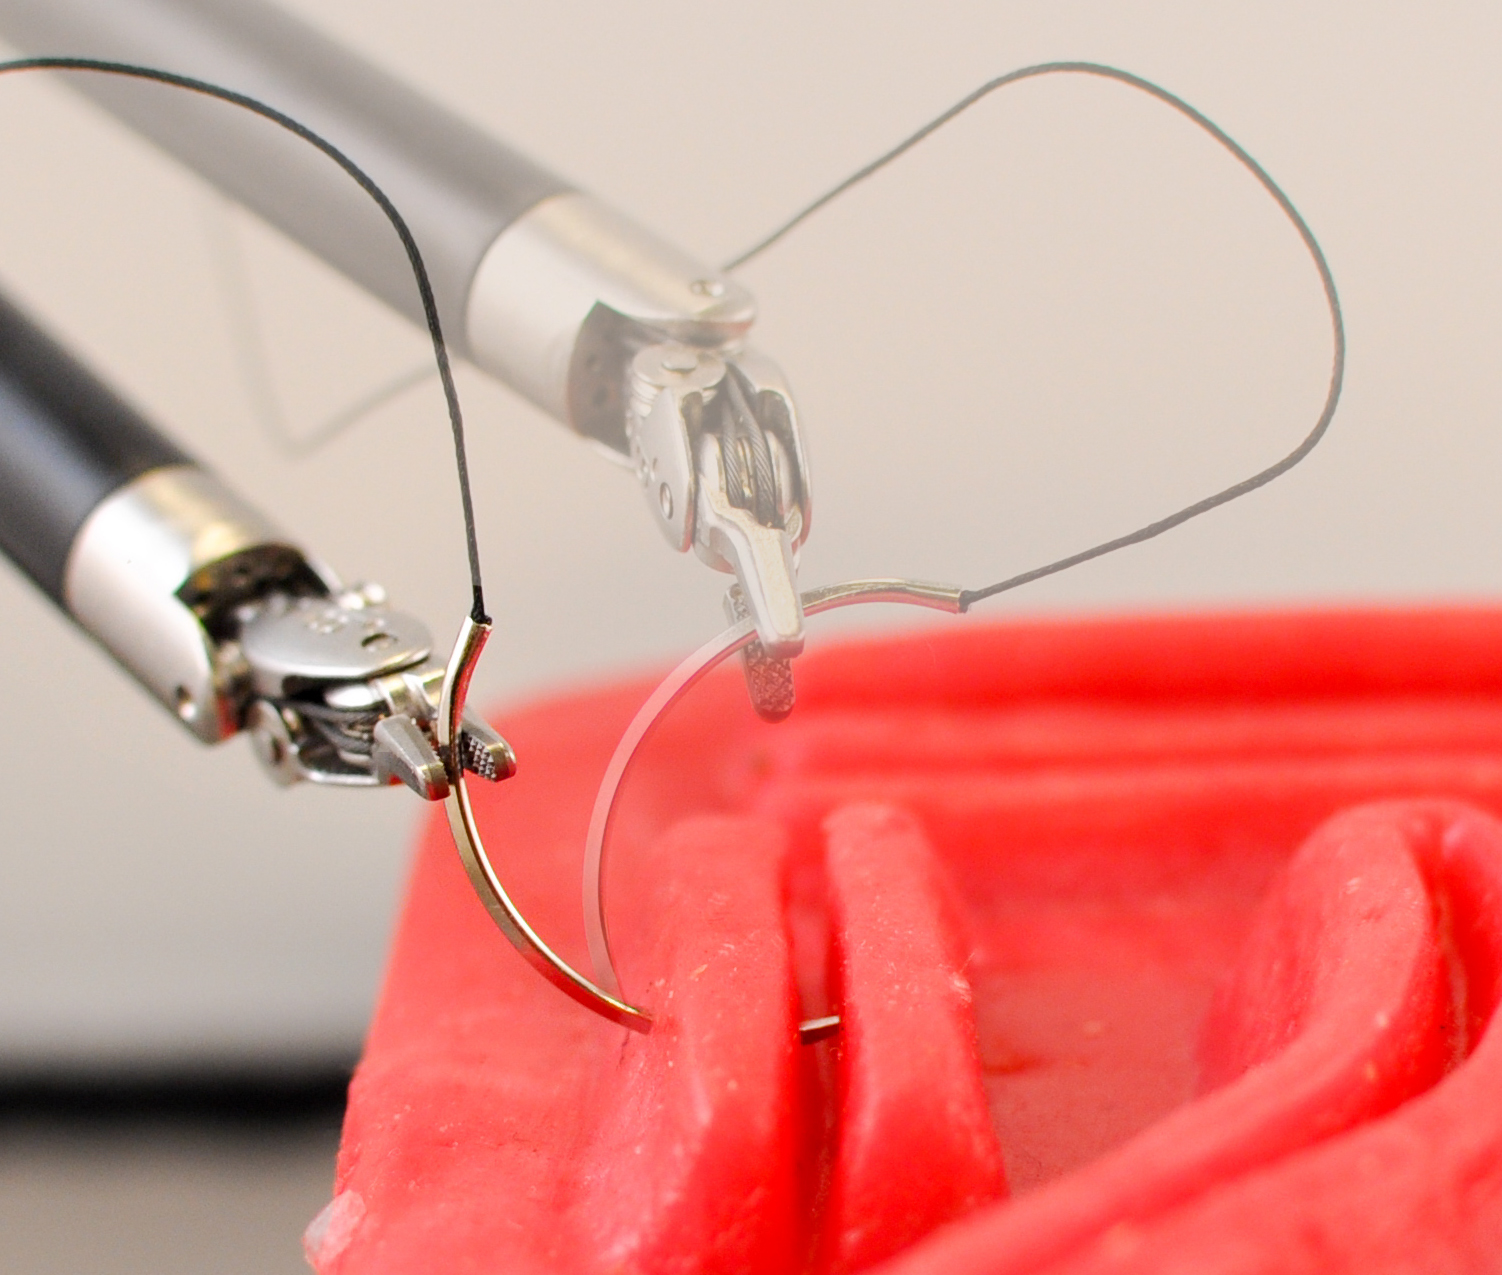
\includegraphics[width=0.9\linewidth]{figures/NeedleInsertionCombo}
% \vspace{-5pt}
\caption{\todo{placeholder} The figure illustrates the steps in autonomous suturing needle insertion step as a time lapse overlay labelled 1, 2, 3, 4. This figure has the complex suturing setup with long running flexible vertical targets. The robot performs [n??] throws of suture in [t??] sec.}
\label{fig:intro}
\vspace{-10pt}
\end{figure}

This paper presents preliminary results towards the automation of the continuous suturing task. We propose a framework of software and hardware that enables robust automation of the continuous suturing task. 
This paper builds upon prior art in optimization based planning with uncertainty\cite{patil2014gaussian},\todo{others}, segmentation of task demonstrations\cite{krishnan2015tsc, lea2015improved}, and building \& tuning finite state machines\cite{Murali2015Learning}. We present a robust segmentation of the single throw suturing task, and build upon the state machine to enable multi-throw running suturing. Each suturing throw is formulated as a curvature constrained trajectory optimization over the pose of the needle leveraging a belief space planning framework. Furthermore, real time needle tracking along with closed loop needle hand-off is demonstrated on the Intuitive Surgical dVRK \cite{Kazanzides2014}. We also present a novel low-cost passive gripper jaw mount for needle alignment. The device allows automatic needle re-positioning, reducing the effort in multilateral needle manipulation to achieve near optimal orientation for needle insertion.

Our system uses an elegant interface allowing the surgeon to trace the wound using the tool tip. Moreover, given one a suture width and a wound depth, the system calculated the required number of suture throws with corresponding entry and exit points. Our system can also be generalized to take a mesh of the incision as a input to the suturing task. The full procedure is performed with closed loop needle tracking and the needle path planner accounts for uncertainty in the needle pose estimation.

\vspace{5pt}
\noindent \textbf{Contributions}:
\begin{enumerate}[noitemsep, leftmargin=*]
\item Robust closed loop Finite State Machine for Continuous Suturing with needle tracking and multilateral needle hand-off. Belief Space Planning based Needle Trajectory Generation and needle size selection.
\item Gripper Jaw mount for automatic needle orientation during grasping for minimizing uncertainty during multilateral manipulation.
\item 4-Throw Continuous Suturing Task as recommended by FRSR~\cite{stegemann2013fundamental}\todo{check paper}. Evaluation on Objective Structured Assessment of Technical Skills (OSATS)~\cite{schreuder2012training} and comparison with manual demonstrations of varying skill levels (expert, intermediates and novices) from the JIGSAWS dataset~\cite{gao2014jhu}. Higher complexity suturing task with vertical walls, evaluation of robustness and time to completion.
\end{enumerate}


\begin{figure*}[!t]
\centering
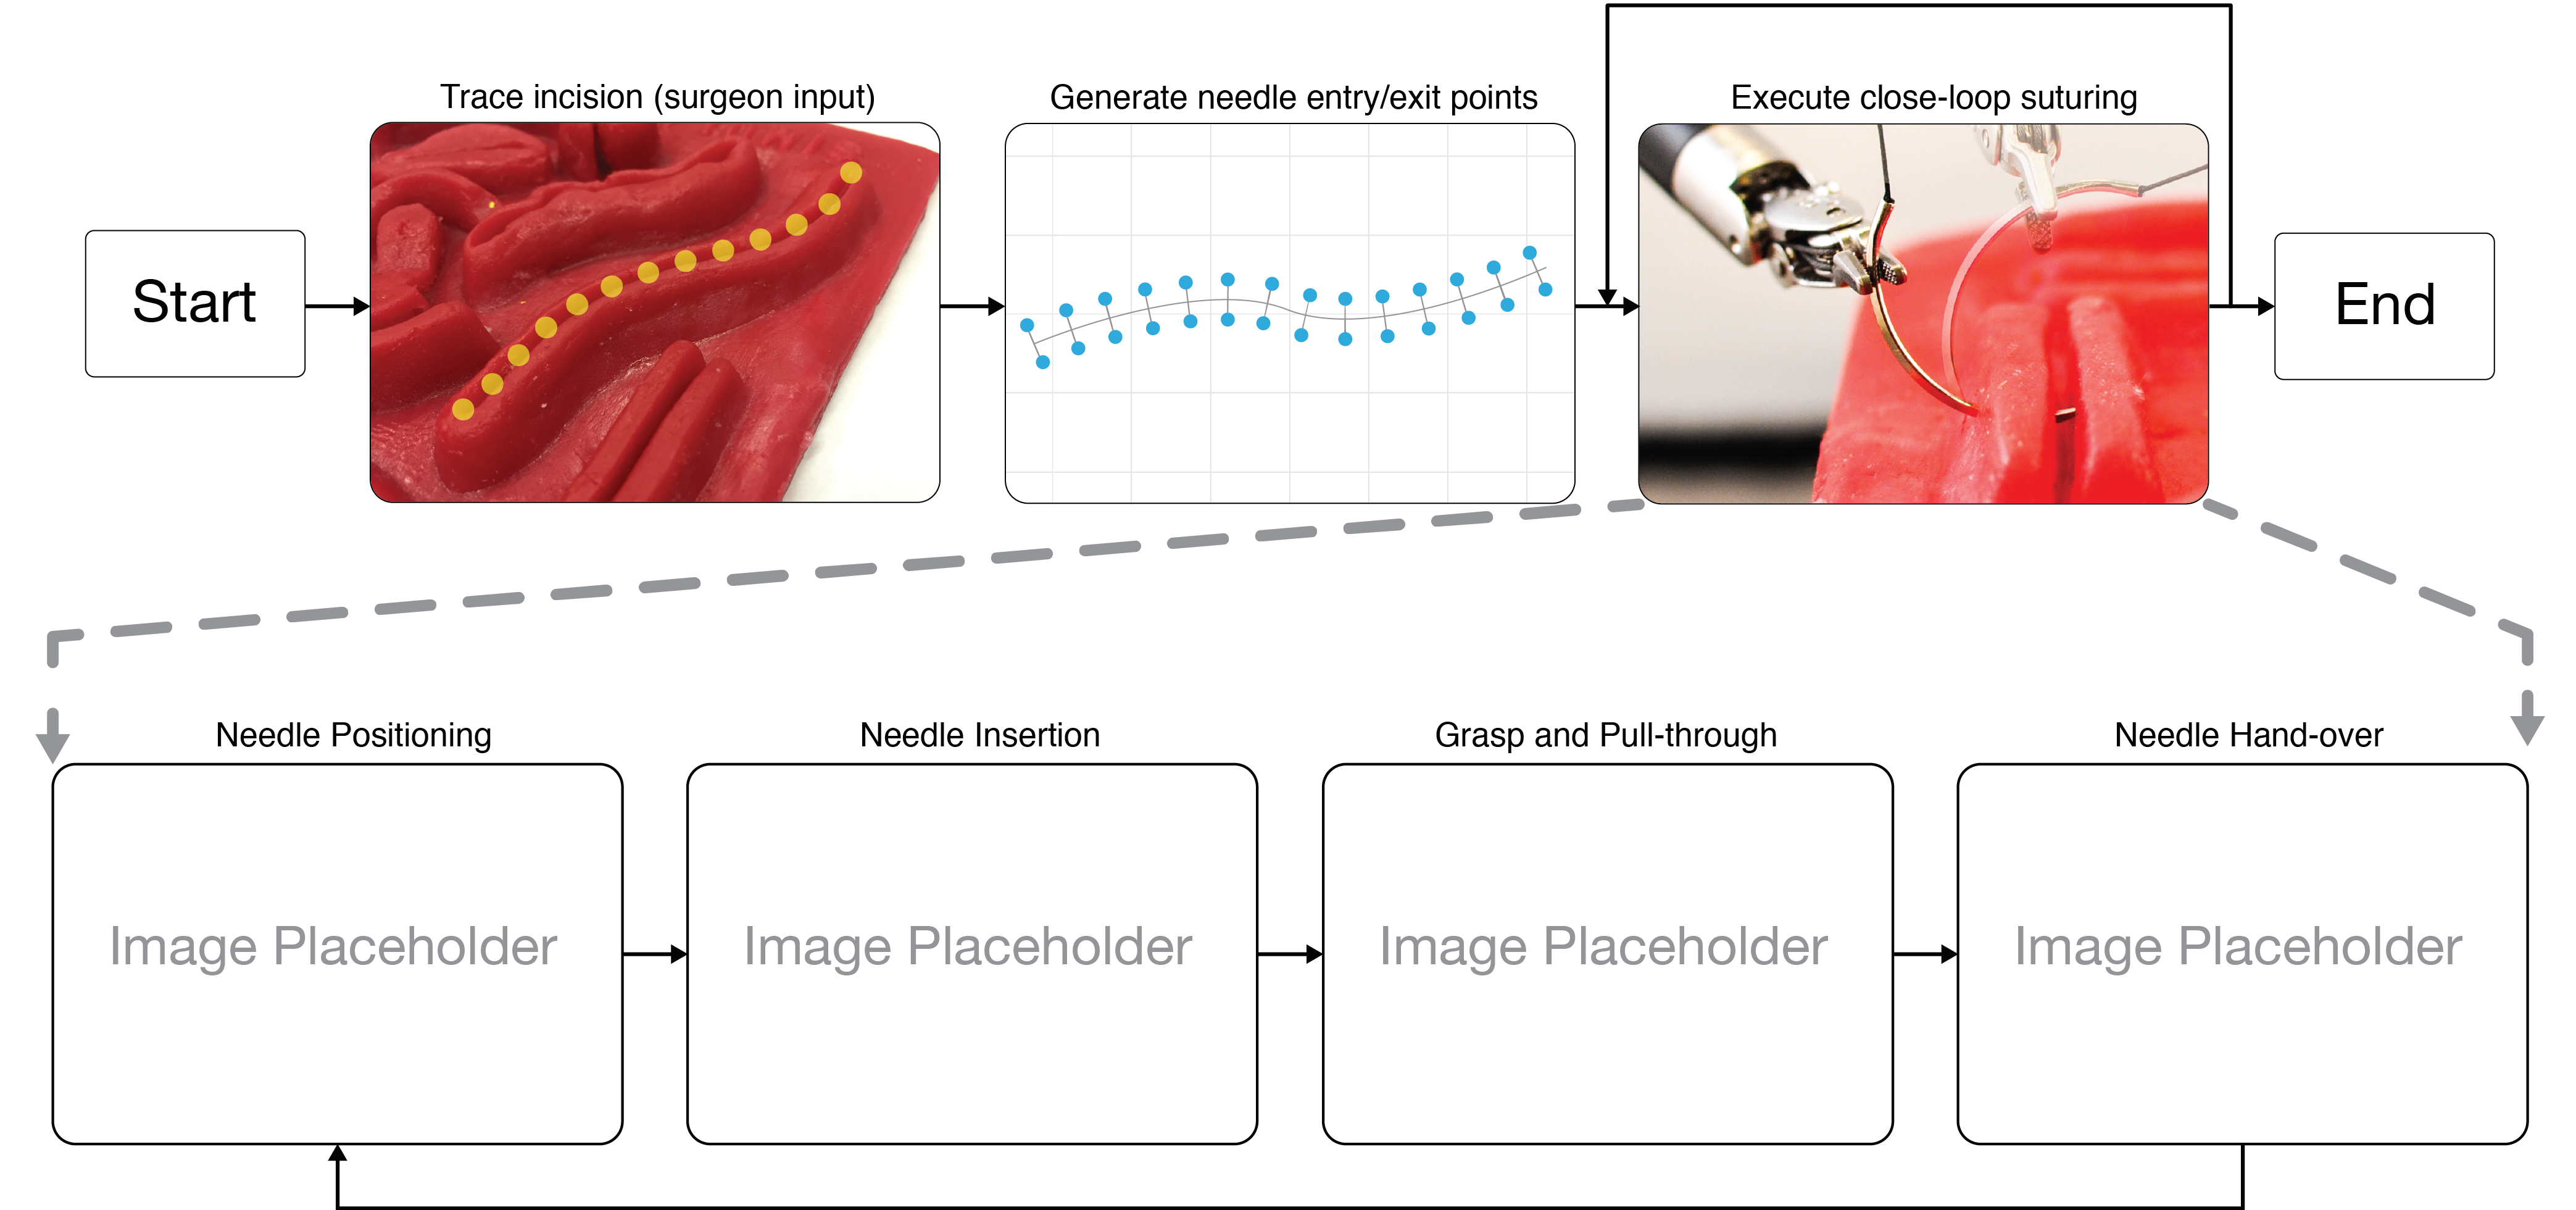
\includegraphics[width=0.9\linewidth]{figures/fsm}
% \vspace{-5pt}
\caption{\todo{Placeholder Figure} The Figure illustrate the algorithmic pipeline.The system receives a trace of the wound to suture along with wound width and depth. Step 2 calculates appropriate number of suture throws and entry/exit points. The suture throws are then repeated until success. Step 3  consists of 4 steps: Needle Positioning, Needle Insertion, Grasp and Pull Through and Needle Hand-off, in accordance with the Manual Labels in the JIGSAWS dataset. Needle Positioning and Needle Insertion is planned using Needle Path Planner, and Needle Grasp and Needle hand-off steps are performed under closed loop operation with needle tracking.}
\label{fig:fsm}
\vspace{-10pt}
\end{figure*}

%==START SECTION==============================
\section{Related Work}
\label{sec:relWork}
%============================================
% Robot assisted surgical systems have been used in a number of surgical interventions~\cite{alterovitz2008motion,Beasley2012,Taylor2008,Wolf2009}.
% Autonomous control of surgical robotic platforms may offer enhancements such as higher precision, higher speed, and lower tissue damage.

% As these authors summarize, contemporary RSA's primarily act as surgical extenders operated directly by the surgeon at all times and may extend human capabilities. Autonomous robotic systems beyond surgical extenders are largely at the experimental level.
% Although academic availability of RSAs such as \textit{Intuitive Surgical} dVRK~\cite{Kazanzides2014} and the Raven II~\cite{hannaford2013raven} system have accelerated recent developments. Task-level autonomy in repetitive and kinematically difficult tasks such as tissue dissection, and suturing may reduce fatigue and operative time. 




% \noindent \textbf{Related Work in Robotic Surgical Automation:}\\
Robot assisted surgical systems have been used in a number of surgical interventions~\cite{Taylor2008,alterovitz2008motion,Wolf2009,Beasley2012}.
Moustris et al.~\cite{Moustris2011} and Kranzfelder et al.~\cite{kranzfelder2013toward} have reviewed recent developments in semi-autonomous and autonomous execution of various surgical procedures. 
Further algorithms for active exploration in tumor localization~\cite{Nichols2013Autonomous}, and tumor ablation~\cite{Hu2015Semi} have also been explored. Our previous work~\cite{Kehoe2014Autonomous} used motion planning to perform multilateral surgical debridement using the Raven II surgical robot.

Surgical training in residents is evaluated using a basis set of  procedures~\cite{stegemann2013fundamental}, the \textit{Fundamental Skills of Robotic Surgery~(FSRS)}, that are representative of frequent sub-tasks experienced by most robot-assisted laparoscopic surgeons~\cite{Ritter2007,dulan2012developing, stegemann2013fundamental}. 
% As described Stegemann et al., the skills can be classified in four groups: (a) Basic Console operation, (b) Psychomotor Skills, (c) Basic Surgery Skills and (d) Intermediate Surgery Skills. ~\cite{stegemann2013fundamental}
It is often observed that procedures are composed of long sequences of subtasks, which are not directly amenable to automation.
Such multi-step procedures can be divided into simpler sub-tasks. 
Hence taking a step towards automation in the context of surgery, Hager et al. proposed a ``Language of Surgery" with ``surgemes" analogous to phonemes~\cite{Lin2006,Reiley2009,Varadarajan2009}.

This has led to a line of work in segmentation of demonstrations into meaningful motion sequences has been extensively studied~\cite{Konidaris2011,Niekum2015,Gienger2010, lea2015improved}. Manual segmentation of surgemes in demonstrations have been used for understanding and recognizing surgical skills and sub-tasks, and for evaluating surgeon skills~\cite{Reiley2009,Varadarajan2009}.
Our recent results on segmentation of task demonstrations~\cite{krishnan2015tsc} demonstrates that unsupervised recovery of semantic transitions is feasible and can be analyzed to construct Finite State Machines~(FSM) for these multi-step procedures.
\citet{Murali2015Learning} showed that finite state machines can be built with a learning by observation approach for robust automation in surgical subtasks involving cutting by provisioning for failure recovery behavior.

\vspace{3pt}
\noindent\textbf{Automation of Suturing: }
Suturing and knot tying have been explored on various occasions in recent past. Starting in early 2000s, \citet{Kang2000Autonomous} developed mathods that focused on the low level control necessary
to automate surgical subtasks such as suturing and knot tying.
Later on, \citet{Mayer2006System} used a recurrent neural net as part of a controller to learn knot tying motion primitives from human demonstrations.\citet{Berg2010Superhuman} used iterative learning control to extract smooth trajectories for performing knot tying at super human speeds. More recently, \citet{Schulman2013Case} used a learning by demonstration approach to warp recorded
expert demonstrations and performing suturing using a simulation of the Raven II. And \citet{Padoy2011} demonstrated execution of a human-robot collaborative suturing task on the DVRK platform. \todo{differentiate from padoy}

% \subsection{Related Work in Motion Planning in Medical Applications}
\vspace{3pt}
\noindent \textbf{Need for planning in suturing: }
One of the main consideration in suturing is minimizing trauma while approximation of the wound. And the choice of needle is very important in it. The needle is chosen based on the \textit{bite length}, the chord length of the needle and \textit{bite width}, conveying the curvature of needle. The objective while suturing is to create an \textit{eversion} in the wound (outward facing bulge) to assist in healing\tocite without applying excessive local force to prevent necrosis. Surgeon best practices require a needle to "bite" the tissue orthogonally during insertion. Additionally, the needle must inserted along a constant curvature arc defined by the shape of the needle in order to minimize trauma to the neighboring tissue \cite{Jackson2013Needle}. These motion constraints are difficult for even expert surgeons to satisfy \cite{Kang2000Autonomous}.

Thus, suturing success is highly dependent on dexterity in needle handling. Incorrect placement of the needle in the gripper may result in a bent needle, difficult penetration of the skin, or an undesirable angle of entry into the tissue. And beyond the correct grasp, the trajectory for a good suture requires complex handling and movement along the curvature of the needle.

\citet{Jackson2013Needle} used surgeon best practices as reference to plan needle paths for suturing, but experimented without uncertainty for a single throw of a given needle. Since the needle tip is moving along a curved path to accommodate the needle curvature, path planning should account for curvature constraints. Recent results in motion planning have shown that optimization based planning is both faster and solver more instances of problems compared to sampling based planners.
Of particular mention is TrajOpt~\cite{Schulman2014Motion} that uses sequential convex optimization to generate locally optimal trajectories.
\citet{Duan2014Planning} leveraged trajOpt to generate curved paths for steerable needle path planning without uncertainty in simulation.

However, as with any real system, there are unmodeled uncertainties in gripper-needle and needle-tissue interactions, which can result in needle to drift from a plan. Hence, tracking needle pose under uncertainty and trajectory plans to account for future uncertainty in control-action mapping can improve robustness. 
Recently, \cite{Kahn2015Active} used belief space optimization to actively explore unstructured environments in order to grasp occluded objects and \cite{Sun2014Motion} developed a motion planner that considers motion and sensor uncertainty while guiding steerable needles in a 3D anatomy.\todo{difference from sun2014motion}
Similarly, there have been explorations on needle tracking for surgical settings as showed by~\cite{wengert2007endoscopic, speidel2015image}.

\vspace{3pt}
\noindent \textbf{Why is our work novel? }
In this work, we use the \davinci Research Kit (dVRK) to perform an end to end continuous suture autonomously. We draw from state-of the art results in both manual labeling~\cite{gao2014jhu} and unsupervised learning of transitions~\cite{krishnan2015tsc}\todo{cite deep paper arxiv version}, to refine them into a robust FSM for the continuous running suturing task with multiple throws.

We segment each suturing throw into a sequence of four surgemes -- Needle Positioning, Needle Insertion, Needle Pull Through and Multilateral hand-off. We address the problem of choosing the correct needle size, positioning and insertion in a joint curvature constrained trajectory optimization problem. 
We use a Lie-Algebra re-parameterization of the pose to improve convergence of the gradient based method.
We also use needle tracking and re-planning to quantify and account for uncertainty using the belief state of the needle in the optimization. 
Use of belief over needle pose in place of deterministic pose, compensates for non-linear interactions with the tissue. Especially since the feedback is not perfect, our approach plans for a conservative path along with a “confidence” in completing the task.

\noindent \textbf{Gripper Augmentation for Needle Orientation: }
Experimental evaluation of the multilateral hand-off procedure needed multiple back and forth passes for achieveing the correct needle configuration in the insertion hand. The procedure still yielded frequent failures due to inaccurate goal poses of needle. To this end, we have devised a novel needle alignment mount for the gripper jaw that passively guides the needle into a known pose upon gripper closure. The device improves needle hand-off accuracy by \todo{x\%} compared to using current needle driver; and hence reduces the need for re-alignment before pushing needle in tissue.  

Automation can be highly beneficial in suturing with a reparametrization the complex motions necessary to effectively perform a stitch. Further, surgical automation can enable semi-supervised surgery by providing surgeons with an ability to input task level commands instead of direct low level control at all points in the surgery. This work is one of the first to present RMIS experiments with autonomous continuous suturing, made possible by a combination of optimization, needle tracking and custom automation enabling hardware.

% supervisory role and high level commands to direct the robot to desired suture locations.

%  Find a better constraint 

% Optimization-based motion planning applied to automating a surgical subtask
% Optimal needle size selection based on surgical environment
% Using lie algebra to optimize over the manifold
% Needle tracking that is robust to partial collusions
% Closed-loop automation of continuous surgical suturing
% Combine needle-tracking with motion planning
% Close-loop planning for optimal hand-off
% Generation of plans accounting for uncertainty



% Why BSP?
% BSP can allow one to account for sources of uncertainty associated with a surgical environment
% Tissue is highly deformable making predictions or simulations of its behavior very difficult.
% Visual feedback can be very noisy
% objects of interest are small (needles, tooltips)
% highly specular surfaces make it difficult to use RGBD sensors
% Modeling the uncertainty can allow the agent to quantify to compute a measure of “confidence” in completing the task (essential in a surgical environment):
% Type-I: Confidence at goal
% Type-II: chances of intermittent failure (drifts off the successful tube of trajectories)
% At each point have a running estimate of both of these measures and possibly create a composite “Confidence” score.


% We try to quantify and account for uncertainty in surgical domain. 
% We use trajectory optimization in belief space to compute curvature constrained, locally optimal trajectories using sequential convex programming. 
% We propose objective criteria to evaluating the quality of a needle trajectory
% We propose a method for selecting the right needle for a specific suturing task.
% We will demonstrate our work on dVRK.

\end{document}

\documentclass[0-suturing.tex]{subfiles}
\begin{document}

%==START SECTION==============================
\section{Problem Formulation}
\label{sec:problem}
%=============================================
Well established manual suture techniques lay the foundation for robotic suturing. In order to complete an independent surgical suture, several components must be preplanned. First, the needle
must enter and exit the tissue in the proper locations and
orientations. Secondly, the needle path must not put any
unnecessary stress on the tissue. Finally, the needle must be
able to react to any unforeseen obstacles that might impede
the needle’s path.
The challenges in learning to suture are difficulty in needle pose estimation, modelling of needle-tissue interaction and creating trajectory plans for robust long-horizon execution. 

% warp the reference needle trajectory
% the reference trajectory is the goal and we want to use motion planning to generate a new trajectory that is close to the reference but minimizes some objective
% incorporate grasp uncertainty into motion plan
% use belief space planning to generate more robust needle trajectory 
\subsection{Suture placement}
The surgeon provides as input a desired suturing line through robotic tele-operation by tracing the tip of the robot's tool through the desired
suturing channel. Let $\mathcal{M} = [M_1, M_2, \ldots, M_D]$ be the discretized trajectory recorded by the system. The surgeon also provides a desired needle bite length $l$, desired bite depth $d$, and a stitch separation $w$.
The full input to our system then is $S,l,d,w$.
Our system outputs an optimal needle size for the given task and  a finite state machine that uses closed loop sensor feedback to autonomously perform a continuous suture. 

We first describe how needle entry and exit points can be generated from surgeon input. Each way point $S_t$ in the desired suturing line can be parametrized by $S_t \in \mathbb{R}^3$, a 3D point. We fit a cubic spline the the series of points to estimate the suturing line. The line is re-sampled such that the distance between each point is $w$ to generate the centers for each stitch in the suture. This can be formalized as the series of points $\mathcal{L} = [L_1, L_2, \ldots, L_F] $ where $ \|L_{i+1} - L_{i}\|_2 = w, \forall i \in [0, \dots, F-1]$. At each stitch center we can generate entry and exit points using equidistant points on opposite sides of the spline.
For each pair of entry and exit points, we developed a motion planning formulation to generate needle trajectories through the tissue.

\subsection{Needle Positioning and Insertion}
The needle's trajectory through the tissue can be discretized into time intervals. Given the entry point of the needle $p_i$, the exit point of the needle $p_f$, we would like to plan a needle motion plan between the two points. Based on the desired bite depth of the stitch, we can generate an avoidance volume below and and above the trajectory. By avoiding collisions with these volumes, we can generate trajectories that allow for successful tissue apposition.



\begin{figure}[t]
\centering
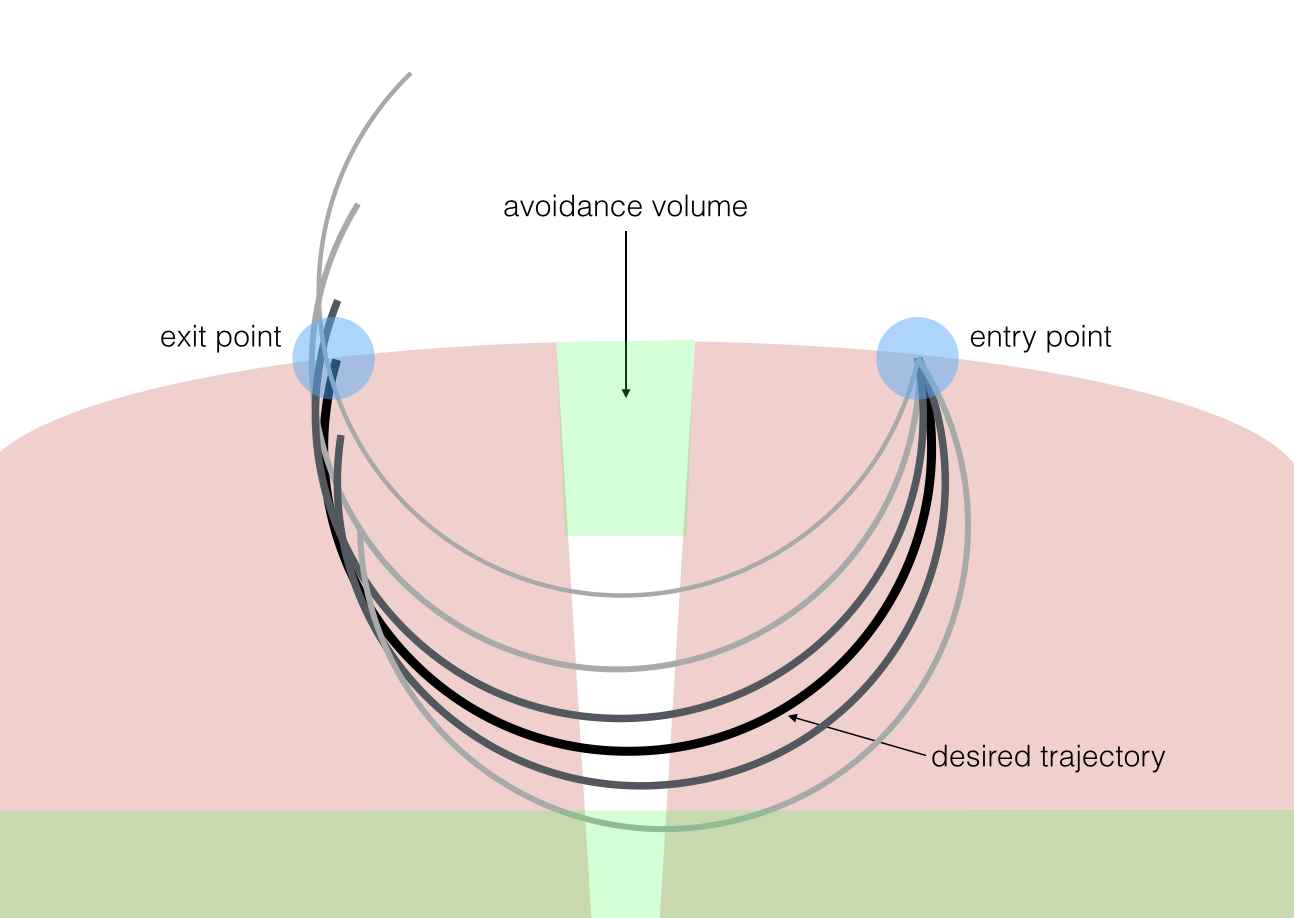
\includegraphics[width=0.85\linewidth]{figures/problem_image.jpg}
% \vspace{-5pt}
\caption{\todo{Placeholder} The is an illustration of a simulated trajectory as it is planned for a given set of parameters.}
\label{fig:toyEx}
\vspace{-15pt}
\end{figure}


\noindent{\textbf{Input:}}\\
We 
Avoidance volume: $\mathcal{O}$ \\
Desired entry point: $p_i$ \\
Desired exit point: $p_f$ \\

\noindent{\textbf{Output:}}\\


\noindent{\textbf{Assumptions:}}\\
- homogeneous tissue\\
- no FEA and tissue interaction model is used to model 
% \noindent{ \textbf{Optimization:}}\\

% some $\Delta$ values to very large numbers while others to zero, resulting 
\subsection{Evaluation Metric}
Performance of closed loop suturing will be measured by\\
- accuracy of needle tracking \\
- accuracy of one throw suturing \\
- accuracy of hand-off \\
- robustness to multi-throw suturing.
\todo{flesh out}


\begin{figure}[!t]
\centering
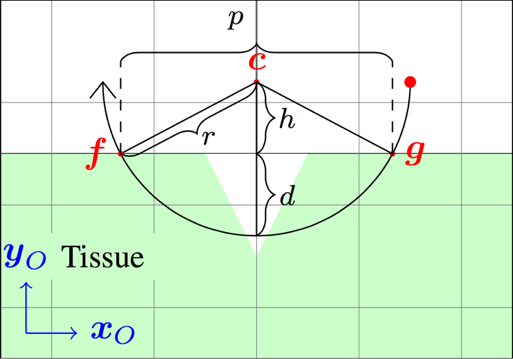
\includegraphics[width=0.8\linewidth]{figures/Schematic}
% \vspace{-5pt}
\caption{\todo{Placeholder} This figure illustrates the notation used in the the optimization problem \todo{refer}}
\label{fig:notation}
\vspace{-10pt}
\end{figure}


%==START SECTION==============================
% \subsection{Our Approach}
%==START SECTION==============================
\section{Proposed Algorithm}
\label{sec:approach}
%============================================
Overview plus block diagram \\

Trajectory Optimization
We use sequential quadratic programming to solve our nonlinear constrained optimization problem
Planning directly in SE(3) is hard
Convex opt works well in flat euclidean spaces
Possible pose representations:
3D+YPR
good: minimal state representation
bad: discontinuities in YPR, gimbal lock
3D + quaternions, 4x4 homogeneous matrix
good: jacobians are always well defined, quaternion work well in many cases
bad: lots of free variables (optimization can get stuck moving along degenerate solutions)
Better solution: optimize on the manifold using the lie algebra (note: used by others as well)
for each iteration of the optimization create a local coordinate parameterization
take gradient steps in $\mathfrak{se}$(3)
convert solution back to SE(3)
repeat for each iteration


\end{document}

\documentclass[0-suturing.tex]{subfiles}
\begin{document}

\section{Needle Path Planning}
\noindent \textbf{Optimization Model}

The trajectory is discretized into time intervals $\mathcal{T} = \{0,1,\ldots,T\}$.


$\mathcal{T} \in [0, 1, \ldots, \mathcal{T}]$.
At each time step the needle's pose is parametrized as
$X_t = \begin{bmatrix}
    R_t & p_t \\ 0^T & 1
\end{bmatrix} \in SE(3)$
where $R_t \in SO(3)$ is a rotation matrix and
$ p_t \in  \mathbb{R}^3 $ is a position.

The control input is parametrized by the needle's radius $r_k$ and the distance $\Delta$, by which the needle is inserted at each time step. We note that $r_k$ is chosen from a discrete set available needle radii. And while $\Delta$ can be selected to be different for each time step, prior empirical results show that the optimization result in uneven distribution of $\Delta$ at each time step resulting undesirable trajectories.


\begin{align}
& \underset{\mathcal{X},\, r_k,\, \Delta}{\text{minimize}}
& & \alpha_\Delta \mathcal{C}_\Delta + \alpha_{Entry} C_{Entry} \\
& \text{subject to}
& & f_{collision}(\mathcal{X}_t, \mathcal{O}) > d_{safe}, & \forall t  \\
& & & curve(\mathcal{X}_{t+1}, \mathcal{X}_t) = r_k, & \forall t  \\
& & & \|p_i-p_1\|_2^2 < \epsilon \\
& & & \|p_f-p_T\|_2^2 < \epsilon \\
& & & T \Delta - 2 \pi l_{max}r_k - 2l_{gripper} < 0 
\end{align}

The costs and constraints in the above formulation are described below:

\subsubsection{Kinematic Constraints (Eq. (3))}
In order to minimize tissue damage, optimal needle trajectories should follow constant curvature paths through tissue. This condition is enforced by ensuring the curvature between timesteps along the trajectory remain 
constant. The constrained can be expressed expressed using Lie algebra defined on the SE(3) group described in the next section.
\begin{equation}
    X_{t+1} =  \text{exp}(\hat{\omega}) \cdot X_{t}
\end{equation}
Where $\omega = \begin{bmatrix} 0 & 0 & \Delta & \Delta r_k & 0 & 0\end{bmatrix}$.
This expression can be transformed into a standard non-convex equality constraint using the matrix log map:
\begin{equation}
    \log(X_{t+1} \cdot (\text{exp}(\hat{\omega}) \cdot X_{t})^{-1})^{\vee} = 0_6   
\end{equation}

\subsubsection{Collision Constraint (Eq. (2))}
We impose constraints to ensure that our trajectory avoids collision with a pre-defined avoidance volume.
This is a mesh can be constructed suture characteristics(width, depth) provided by a surgeon. Our technique
also allows this mesh to be general and non convex. This would allow mesh construction from visual inputs from sensory tools such as endoscopic cameras or ultrasound.  Hierarchical Approximate Convex Decomposition(HACD) \todo{cite} is used to decompose a given avoidance volume into a set of convex meshes 
$\mathcal{O} = \{O_1, \ldots, O_m\}$. We avoid collisions by ensuring that the signed distance between each 
point in the trajectory and each convex mesh in $\mathcal{O}$ is greater than a user defined safety margin $d_{safe}$. 


\subsubsection{Entry and Exit Point Constraints (Eq. (4) and (5))}
We define a maximum allowable error in $l_2$ distance $\epsilon$ for the start and end points of our trajectory.


\subsubsection{Needle Length Constraints (Eq. (6)) }
Our optimization needs to generate needle trajectories that are feasible within the physical dimensions of the needle. \todo{rephrase this}. 
The length of the trajectory can by approximated as $T\Delta$. In order to perform a successful needle insertion and pull through, the needle length needs to be longer than the trajectory length, and the two gripper widths. 
The maximum length of a needle is defined by the radius of curvature of the needle and the proportion of a full circle the needle's arc carves out. 
For most surgical applications needle arcs are either $\frac{3}{8}$, $\frac{1}{2}$, $\frac{5}{8}$ of a full circle. 
Thus we can define our max needle length as $2 \pi l_{max}r_k$ where $l_{max} = \frac{5}{8}$.
The full constraint then is reformulated in standard form in equation 6.


\subsubsection{Costs (Eq. (1))}
To penalize tissue damage we opimize for the smallest needle trajectory that satisfies our constraints.
We approximate the trajectory length as:
\begin{equation}
    C_{\Delta} = T\Delta 
\end{equation}
Surgical best practices suggest that needles should enter the tissue surface in a direction close to the surface normal.
We can use the lie algebra to express the constraint as the following:
\begin{equation}
    C_{Entry} = \|\log(X_f \cdot X_T^{-1})^{\vee}\|^2_2
\end{equation}


\subsection{\textbf{Re-parametrization of Pose Constraints}}
Generating collision-free, constant curvature trajectories in 3D space is challenging because it requires planning in the Special Euclidean Group in 3D, i.e. $SE(3)$ configuration space.
SE(3) is a semidirect product of Special Orthogonal Group (SO(3)) and $\mathbb{R}^3$. Using homogeneous coordinates, we can represent SE(3) as follows:
\begin{equation}
\begin{aligned}
SE(3) &= \left\{
\begin{bmatrix}
R & p \\
0 & 1
\end{bmatrix}
\in GL(4) \rvert R \in SO(3), t \in R^3 \right\}
\end{aligned}
\end{equation}

\noindent The action of an element $g \in SE(3)$ on a point $p \in \mathbb{R}^3$ is given by
$g = \begin{bmatrix}
R & p \\
0 & 1
\end{bmatrix},
\quad g \cdot p = Rp + t $.

% \begin{equation}
% \begin{aligned}
% g &=
% \begin{bmatrix}
% R & p \\
% 0 & 1
% \end{bmatrix} \\
% & g \cdot p = Rp + t
% \end{aligned}
% \end{equation}

Trajectory optimization methods that use sequential convex optimization, iteratively update a trajectory until the all the problem constraints are satisfied and objective function reaches a local minimum. However, optimization directly over the trajectory in pose representation (homogeneous coordinates in our case) can lead to poor results and slow convergence rates.

Rotation parametrizations such as quaternions or rotation matrices are over-constrained and can cause the optimization to be numerically unstable iterating over degenerate solutions.
While on the other hand, axis angle representations have the correct number of degrees of freedom but deformation at the poles of the configuration space severely slows down convergence.

Since $SE(3)$ is a differentiable manifold, we can instead optimize over the manifold using the corresponding Lie algebra, $\mathfrak{se}(3)$, which is defined as the tangent vector space at the identity of SE(3). An excellent introduction in lie algebraic approach in pose registration in provided by~\citet{Agrawal2006Lie}.

\noindent The Lie algebra of $SE(3)$ is given by
\begin{equation}
    \mathfrak{se}(3) = \left\{
    \begin{bmatrix}
        \hat{\omega} & u \\
        0 & 0
    \end{bmatrix}
    \in GL(4) \rvert \hat{\omega}\in so(3), u \in \mathbb{R}^3
    \right\}
\end{equation}

\noindent Here $\hat{\omega}$ is the skew symmetric form of the rotation vector
$\omega = (\omega_x, \omega_y, \omega_z)^T$ and is an element of the Lie algebra for $SO(3)$
\begin{equation}
    \hat{\omega} =
    \begin{bmatrix}
        0 & -\omega_z & \omega_y  \\
        \omega_z & 0 & -\omega_x \\
        -\omega_y & \omega_x & 0
    \end{bmatrix}
\end{equation}

\noindent The logarithm map $SE(3) \to \mathfrak{se}(3)$ is given by:
\begin{equation}
    \text{log}\left(
        \begin{bmatrix}
            R & t \\
            0 & 1
        \end{bmatrix}
    \right)  =
    \begin{bmatrix}
        log(R) & A^{-1}t \\
        0 & 0
    \end{bmatrix}
    \label{eq:logMap}
\end{equation}

\noindent where
\begin{equation*}
\begin{aligned}
    A^{-1} &= I - \frac{1}{2}\hat{\omega} +
\frac{2\sin\|\omega\| - \|\omega\|(1+cos\|\omega\|) }{2\omega^{2} \sin\|\omega\|}\hat{\omega}^{2},  \\
log(R) &= \frac{\phi}{2sin(\phi)}\big(R - R^T\big) \equiv \hat{\omega}
\end{aligned}
\end{equation*}
and $\phi$ satisfies $Tr(R) = 1+2cos(\phi), \quad |\phi|<\pi$.
\vspace{5pt}
\noindent The matrix exponential to map $\mathfrak{se}(3) \to SE(3)$ is given by
\begin{equation}
    \text{exp}\left(
        \begin{bmatrix}
            \hat{\omega} & u \\
            0 & 0
        \end{bmatrix}
    \right)  =
    \begin{bmatrix}
        \text{exp}(\hat{\omega}) & Au \\
        0 & 0
    \end{bmatrix}
    \label{eq:expMap}
\end{equation}

\noindent where $\text{exp}(\hat{\omega})$ can be computed with Rodrigue's formula:
\begin{equation*}
\begin{aligned}
    \text{exp}(\hat{\omega}) &= I + \frac{1-\cos(\|\omega\|)}{\|\omega\|}\hat{\omega}^2 +
    \frac{\sin(\|\omega\|)}{\|\omega\|^2}\hat{\omega},\\
    A &= I + \frac{1-\cos(\|\omega\|)}{\|\omega\|^2}\hat{\omega} + \frac{\|\omega\| - \sin\|\omega\|}{\|\omega\|^3}\hat{\omega}^2
\end{aligned}
\end{equation*}

With equations \eqref{eq:logMap} and \eqref{eq:expMap}, we can convert an element in SE(3) to $\mathfrak{se}(3)$ and vice-versa. Furthermore, we can also \todo{Jacobians}

\subsection{Modelling Uncertainty }
\todo{fill out the bsp formulation.}
Write about how to use the equations of the covariance matrix in the optimizaiton formulation using analytical derivatives.



\subsection{Suturing Best-Practice for Initialization}
\todo{rephrase and quantify}
There are many general rules that surgeons use to complete
a suture. A typical list of such rules is below [10] [11].
Manual needle sutures normally result in a picture similar to
Fig. 1.
1. The needle first “bites” the tissue orthogonally. By
inserting the needle such that the tip is orthogonal to
the tissue surface, tissue surface stress is minimized.
2. The wrench between the tissue and the needle during
the suture must be minimized. Minimizing the needle
tissue interaction force reduces the internal tissue stress,
and consequently reduces additional tissue trauma due
to the suture.
3. The re-grippable length of the needle during the
suture must be adequate for the needle re-grasp to be
completed successfully. Since the needle holder can
not be inserted through the tissue, there must be an
intermediate point during the suture that the gripper can
regrasp the needle on the tip to complete the suture.
4. The final depth of the needle in the tissue is an
important component of a successful suture. The actual
target depth is determined by many factors, including
both the wound being closed and the size of the needle.
5. The needle tip should only touch the tissue at the
insertion site. Similarly, the needle gripper should not
place unnecessary stress on the tissue.
The above list is not exhaustive, but details important components
of a quality suture.
Converting the listed suture principles into a list of analytic
equations allows for the planning algorithm to be automated
and optimized against the suture guidelines.

\end{document}

\documentclass[0-suturing.tex]{subfiles}
\begin{document}

\section{System Design}
\label{sec:system}
\subsection{User Interface for wound tracing.}
describe the simple interface here

 dVRK is a research platform built from mechanical components from the first-generation of the \davinci surgical system \cite{Ballantyne2003} and electronics and software from WPI and Johns Hopkins University~\cite{Kazanzides2014}.

\subsection{Multilateral Hand-offs for Optimal Needle Re-orientation}
describe the search method here.  


\subsection{Needle Tracking}
Block diagram for the approach along with real images. 
some explanation of the math, and cite CPD2 for affine point registration. 
step by step.

Needle Tracking

    We use paint to color our needles yellow so that we can use HSV thresholding to
segment the needles. We apply an erosion filter to the image to remove noise and
outlier pixels from segmented image. Next we use point set registration to fit an
elliptical arc to the segmentation mask. We use the CPD2 algorithm to find
an affine transformation which when applied to a circular arc, best fits our
segmentation. This process in repeated in our left and right camera images and
correspondence points are used to generate 3D points along the needles.
The end points are used to generate a pose on the the left and right edges of
the needle. We apply a kalman filter to smooth our pose estimates.
Our needle alignment tool tips ensure that the needles lie on a known plane when
they are held by the grippers. We project our gripper estimates onto this known
plane to improve the robustness our estimates.
    Since the point set registration algorithm is robust to outliers and missing
data, the needle can still be tracked in instances when it is partially oclluded.
Partial ocllutions occur whenever the needle is being held in a tool or when it
is inserted into tissue. Both are instances when needle tracking is necessary
for closed loop control. Furthermore, specularies and changes in lighting conditions
cause cause the HSV segmentation to be incomplete - resulting in needle masks
containing holes. Our technique allows us to interpolate points along the needle
in these holes.




\begin{figure}[!t]
\centering
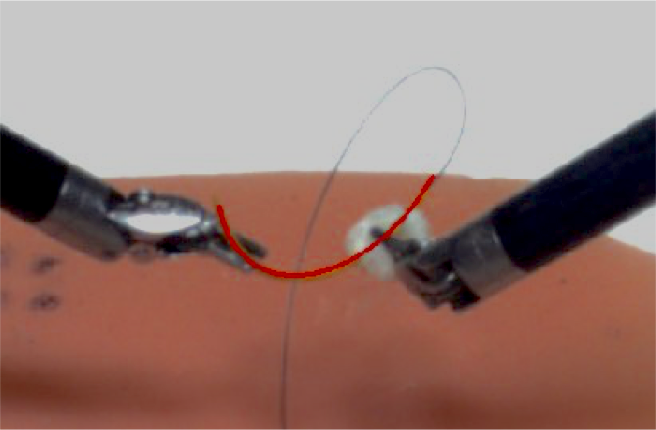
\includegraphics[width=0.9\linewidth]{figures/needleTrack}
% \vspace{-5pt}
\caption{\todo{Placeholder}The figure illustrates our needle tracking system along with the algorithm used. This system can successfully track needle pose through partial occlusions such as when needle is parially inside tissue and gripper occlusions during hand-offs.}
\label{fig:tracking}
\vspace{-10pt}
\end{figure}


\subsection{Design of a Needle Driver Jaw Attachment to Facilitate Pose Orientation}

A difficulty faced in the automation of suturing is the uncertainty of needle pose \tocite. Position and orientation of a needle gripped within the \textit{da~Vinci Large Needle Driver} is unconstrained for rotation in two directions and translation along the length of the needle. Although perception of a needle within a surgical workspace is possible using stereoscopic vision \tocite, it is still noisy and uncertain \tocite. Even with perfect perception, additional time consuming steps would be needed to correct the needle's pose. Constraining the orientation of a grasped needle to a single degree of freedom would allow for easier pose estimation as well as fewer pass-offs. Based off of previous work in self righting grippers such as \cite{Articulating needle driver} and 
\cite{Needle holder with suture filament grasping abilities}, the needle gripper attachment was designed to orient a curved needle to a single pose with uncertainly only in translation along the length of the needle. As the grippers approach a needle, the needle is funneled towards a groove running perpendicular to the length of the gripper jaws. Upon closing the jaws, the needle rolls to a single pose of stability between contact points C \todo{add contact points C and J to figure} and jaw J as shown in Figure~\todo{add figure reference}(b) and Figure~\todo{add figure ref}(d).



The front plane of the jaw attachment (area P \todo{add area P to figure} in Figure~\todo{add figure ref}(c)) is designed to provide a collision surface for the approaching needle and is also used as a mechanical constraint for a second Needle Driver during the process of needle passing. The rear wall R shown in Figure~\todo{refer to figure}(a) \todo{add R to figure} is designed to provide a collision surface for an approaching needle. These features (area P and wall R) are designed to overcome needle and Needle Driver pose uncertainty and passively facilitate needle gripping and pose estimation. The size of the needle gripper and the distance between contact points P is dependent on the curvature of the needle; in this case, we designed our gripper specifically for the ½ 36mm needle, resulting in a total width of 10mm.

We fabricated the mount out of ABS plastic using a Stratysys uPrint 3D printer. Due to surface texture of the $3$D-printed surface and the triangular cross-section of the needle, a semi-stable antipodal pose can be achieved if the needle is initially approached 180 degrees from its desired pose. Kinematic or visual feedback can be used to determine if this has occurred, and a re-grasp can be attempted produce the desired results.

\todo{flesh out the second version of design, why is it concave not convex --rather counter intuitive, }

\begin{figure}[t!]
\centering
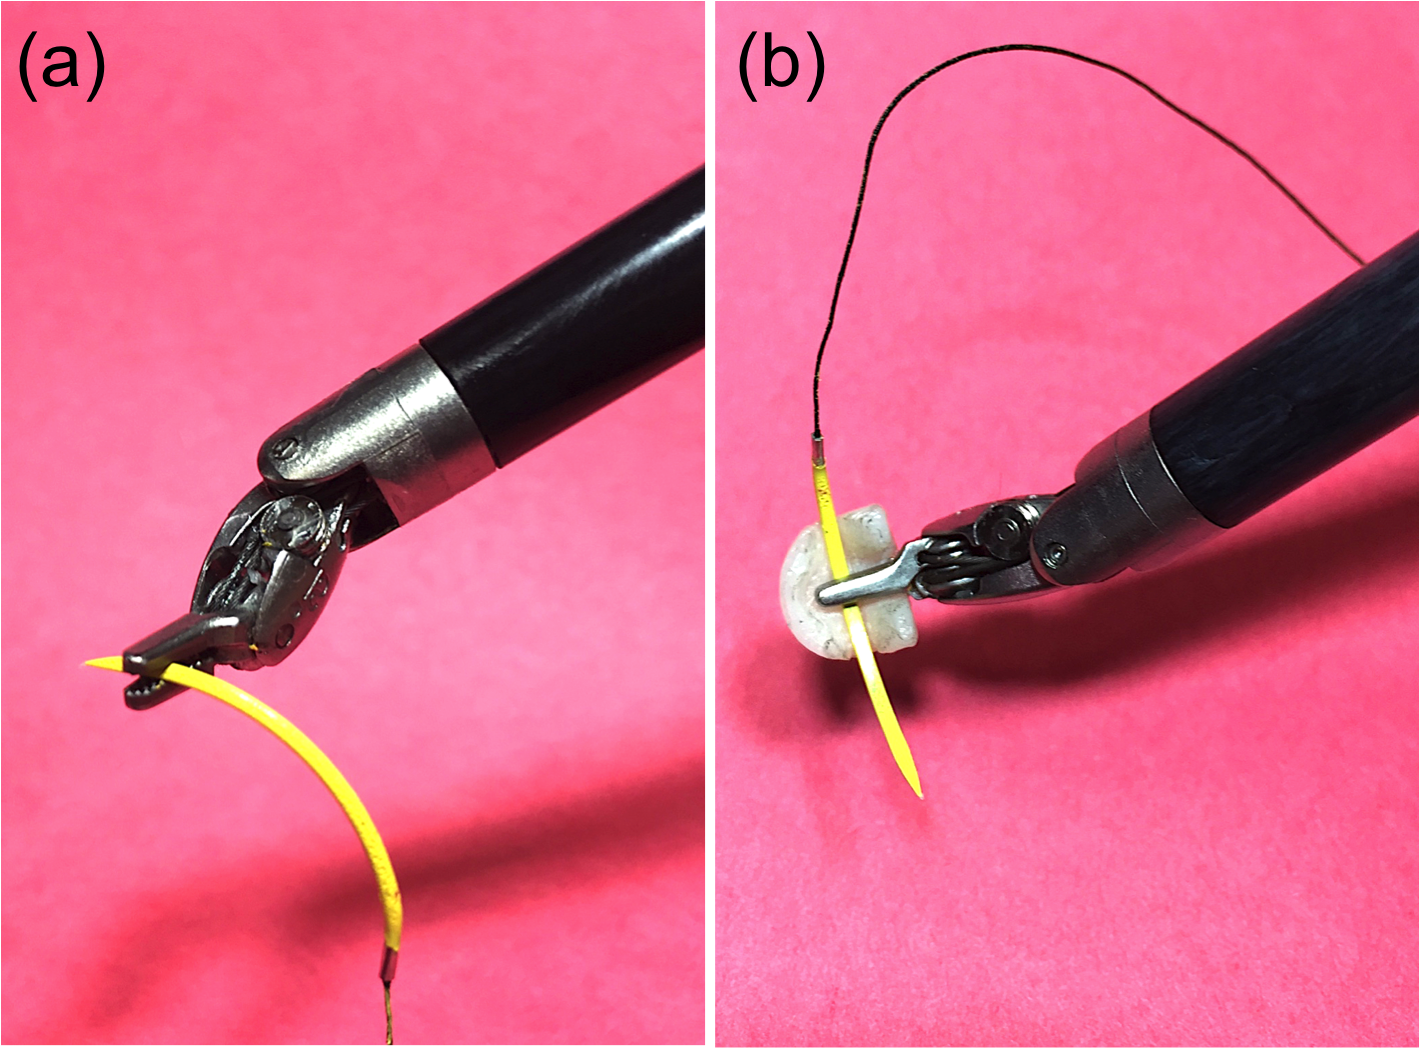
\includegraphics[width=0.95\linewidth]{figures/gripperAttachment}
% \vspace{-5pt}
\caption{\todo{placeholder caption}Figure (a) shows a suboptimal needle orientation both in position and rotation. Figure (b) shows the passive correction in action, with the needle held in correct orientation and position to facilitate insertion. }
\label{fig:jawMount}
\vspace{-10pt}
\end{figure}


\begin{figure*}[!t]
\centering
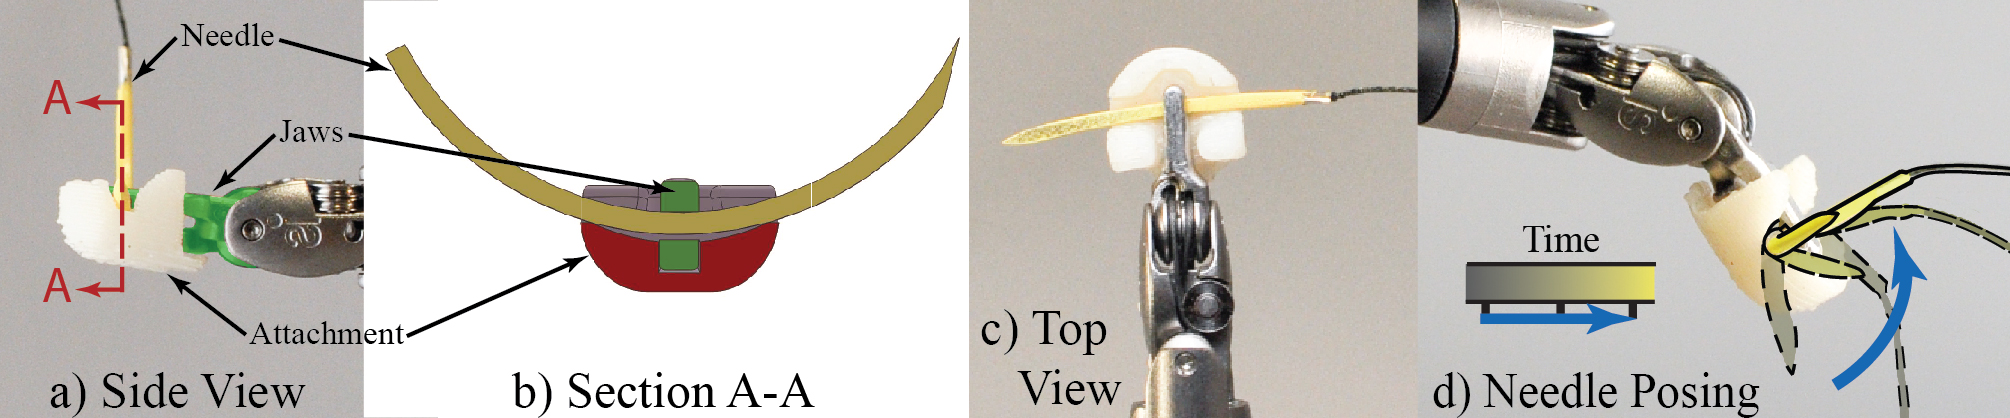
\includegraphics[width=\linewidth]{figures/NeedleGripper2-01}
% \vspace{-5pt}
\caption{\todo{caption}Detail the design of the gripper attachment}
\label{fig:gripper design}
\vspace{-10pt}
\end{figure*}

\subsection{Needle grasp and Pull Through}
describe the strategy in detail. 

\end{document}

\documentclass[0-suturing.tex]{subfiles}
\begin{document}

%==START SECTION==============================
\section{Experiments and Results}
\label{sec:expt}
%===========================================


Experimental Results
Results in simulation
compare state space plan to belief space plan
expect the belief space plan to be more “conservative”
run forward simulations using varying noise models to validate the BSP trajectory
show how varying different costs affects the trajectory
Running on the actual robot
Build incisions using silicon models and test needle trajectories on the robot
Test trajectory sensitivity by varying the phantom’s shape and material properties

\end{document}

\documentclass[0-suturing.tex]{subfiles}
\begin{document}


%==START SECTION==============================
\section{Discussion and Future Work}
\label{sec:discussion}
%============================================


%==START SECTION==============================
\section{Conclusions}
\label{sec:conclusion}
%============================================

\end{document}


% \vspace{-5pt}
\subsection*{Acknowledgements}
\label{sec:ack}
{\small This work is supported in part by a seed grant from the UC Berkeley Center for Information Technology in the Interest of Science (CITRIS), and by the U.S.\ National Science Foundation under Award IIS-1227536: Multilateral Manipulation by Human-Robot Collaborative Systems. We thank Intuitive Surgical, Simon DiMao, and the dVRK community for support; NVIDIA for computing equipment grants; Andy Chou and Susan Lim for developmental grants; and Dr. Walter Doug Boyd for insight and advice and \todo{XX YY} for revising the manuscript.}


\bibliographystyle{IEEEtranN}%ordered refs %also requires natbib-sort&compress
% \bibliographystyle{IEEEtrans}%alphabetical refs
\bibliography{library,palpationCASE,suturing}
\end{document}